%%%%%%%%%%%%%%%%%%%%%%%%%%%%%%%%%%%%%%%%%
% University/School Laboratory Report
% LaTeX Template
% Version 3.1 (25/3/14)
%
% This template has been downloaded from:
% http://www.LaTeXTemplates.com
%
% Original author:
% Linux and Unix Users Group at Virginia Tech Wiki 
% (https://vtluug.org/wiki/Example_LaTeX_chem_lab_report)
%
% License:
% CC BY-NC-SA 3.0 (http://creativecommons.org/licenses/by-nc-sa/3.0/)
%
%%%%%%%%%%%%%%%%%%%%%%%%%%%%%%%%%%%%%%%%%

%----------------------------------------------------------------------------------------
%	PACKAGES AND DOCUMENT CONFIGURATIONS
%----------------------------------------------------------------------------------------

\documentclass{article}

\usepackage[version=3]{mhchem} % Package for chemical equation typesetting
\usepackage{siunitx} % Provides the \SI{}{} and \si{} command for typesetting SI units
\usepackage{graphicx} % Required for the inclusion of images
\usepackage{natbib} % Required to change bibliography style to APA
\usepackage{amsmath} % Required for some math elements 

\setlength\parindent{0pt} % Removes all indentation from paragraphs

\renewcommand{\labelenumi}{\alph{enumi}.} % Make numbering in the enumerate environment by letter rather than number (e.g. section 6)

%\usepackage{times} % Uncomment to use the Times New Roman font

%----------------------------------------------------------------------------------------
%	DOCUMENT INFORMATION
%----------------------------------------------------------------------------------------

\title{Lab Report 4 \\ D-Latch, Flip Flops, 8-bit Register \\ ECE 238L \\} % Title
\author{Kenneth Cox}
\date{\today} % Date for the report

\begin{document}

\maketitle % Insert the title, author and date

\begin{center}
\begin{tabular}{l r}
Date Performed: & April 9, 2021 \\ % Date the experiment was performed
Instructor: & Professor Hamke % Instructor/supervisor
\end{tabular}
\end{center}

% If you wish to include an abstract, uncomment the lines below
% \begin{abstract}
% Abstract text
% \end{abstract}


%----------------------------------------------------------------------------------------
%	SECTION 1
%----------------------------------------------------------------------------------------


% If you have more than one objective, uncomment the below:
%\begin{description}
%\item[First Objective] \hfill \\
%Objective 1 text
%\item[Second Objective] \hfill \\
%Objective 2 text
%\end{description}

\section{Items}

\begin{description}
\item[D-Latch]
\item[Flip Flop]
\item[8-Bit Register]
\end{description} 
 
%----------------------------------------------------------------------------------------
%	SECTION 2
%----------------------------------------------------------------------------------------


\begin{figure}[h]
\begin{center}
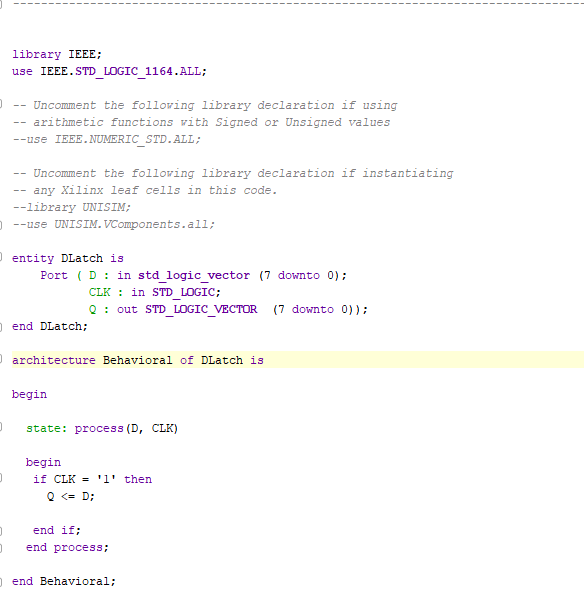
\includegraphics[width=1\textwidth]{DLatchSource.png} % Include the image placeholder.png
\caption{D-Latch Source}
\end{center}
\end{figure}

\begin{figure}[h]
\begin{center}
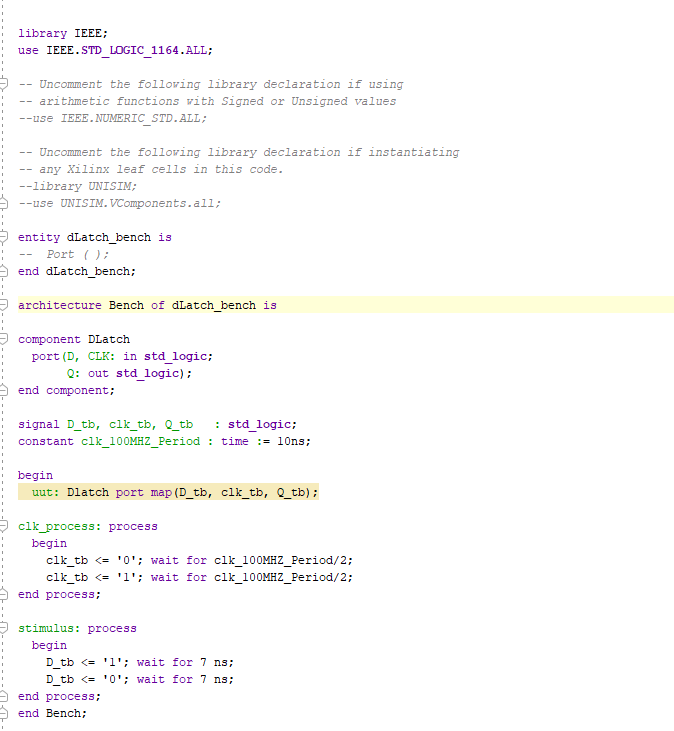
\includegraphics[width=1\textwidth]{DLatchSimSource.png} % Include the image placeholder.png
\caption{D-Latch Test Bench}
\end{center}
\end{figure}

\begin{figure}[h]
\begin{center}
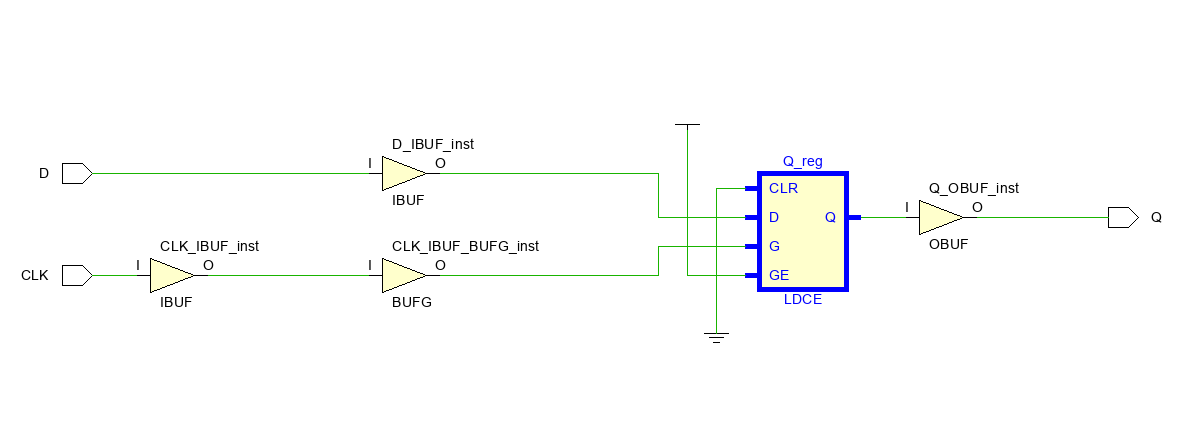
\includegraphics[width=1\textwidth]{DLatchDiagram.png} % Include the image placeholder.png
\caption{D-Latch Schematic}
\end{center}
\end{figure}


\begin{figure}[h]
\begin{center}
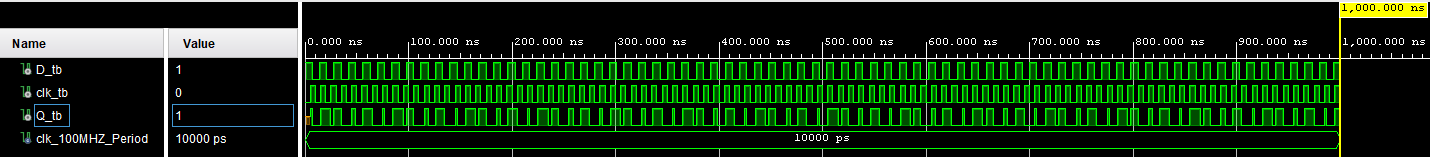
\includegraphics[width=1\textwidth]{DLatchWF.png} % Include the image placeholder.png
\caption{D-Latch Wavefrom}
\end{center}
\end{figure}

%----------------------------------------------------------------------------------------
%	SECTION 3
%----------------------------------------------------------------------------------------

\begin{figure}[h]
\begin{center}
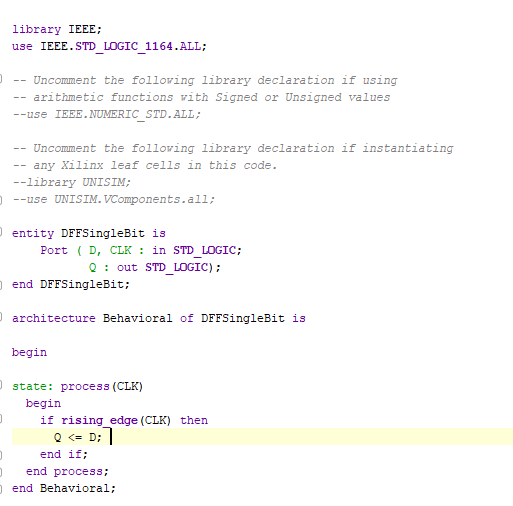
\includegraphics[width=1\textwidth]{FlipFlopSource.png} % Include the image placeholder.png
\caption{Flip Flop Source}
\end{center}
\end{figure}

\begin{figure}[h]
\begin{center}
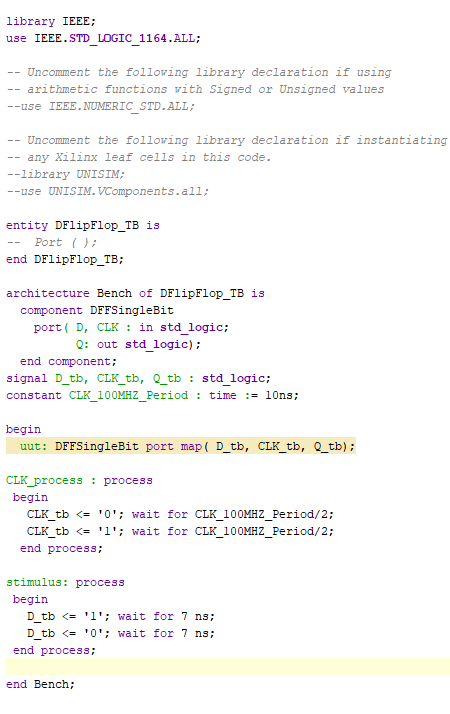
\includegraphics[width=1\textwidth]{FlipFlopSimSource.png} % Include the image placeholder.png
\caption{Flip Flop Test bench}
\end{center}
\end{figure}

\begin{figure}[h]
\begin{center}
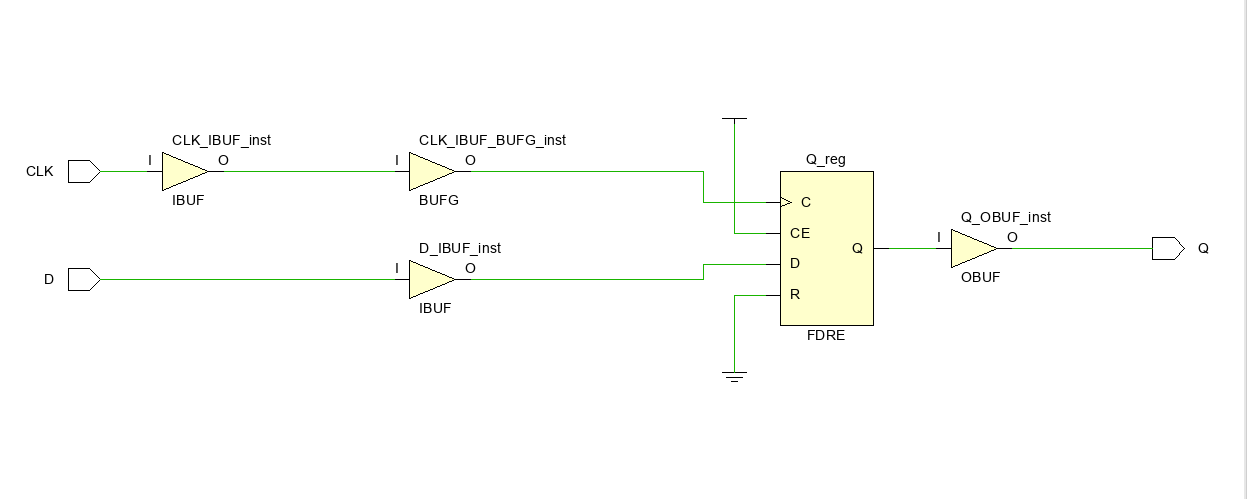
\includegraphics[width=1\textwidth]{FlipFlopSchematic.png} % Include the image placeholder.png
\caption{Flip Flop Schematic}
\end{center}
\end{figure}

\begin{figure}[h]
\begin{center}
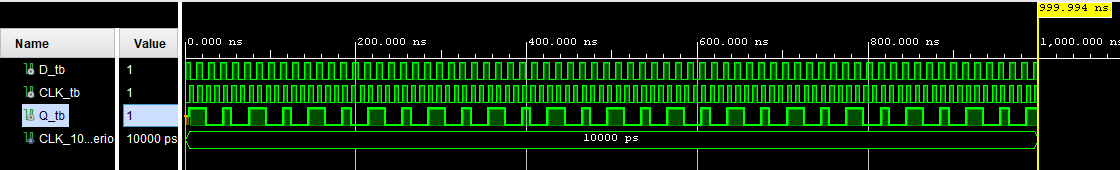
\includegraphics[width=1\textwidth]{FlipFlopWaveForm.png} % Include the image placeholder.png
\caption{Flip Flop Waveform}
\end{center}
\end{figure}

%----------------------------------------------------------------------------------------
%	SECTION 4
%----------------------------------------------------------------------------------------


\begin{figure}[h]
\begin{center}
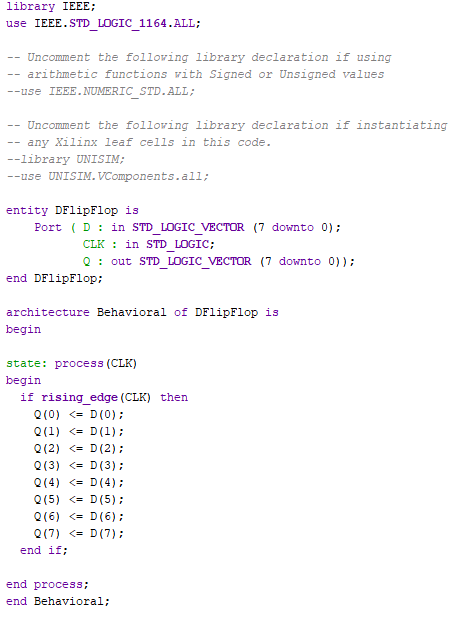
\includegraphics[width=1\textwidth]{8BitRegisterSource.png} % Include the image placeholder.png
\caption{8-Bit Register Source}
\end{center}
\end{figure}

\begin{figure}[h]
\begin{center}
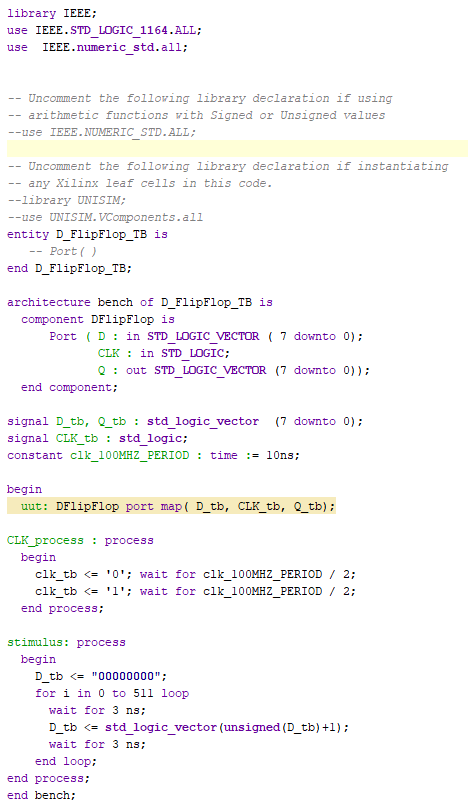
\includegraphics[width=1\textwidth]{8BitRegisterSimSource.png} % Include the image placeholder.png
\caption{8-Bit Register Test Bench}
\end{center}
\end{figure}

\begin{figure}[h]
\begin{center}
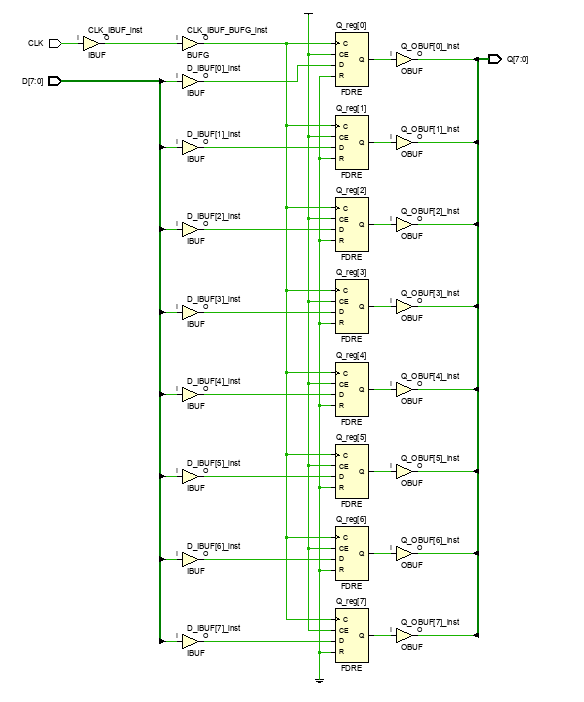
\includegraphics[width=1\textwidth]{8BitRegisterSchematic.png} % Include the image placeholder.png
\caption{8-Bit Register Schematic}
\end{center}
\end{figure}


\begin{figure}[h]
\begin{center}
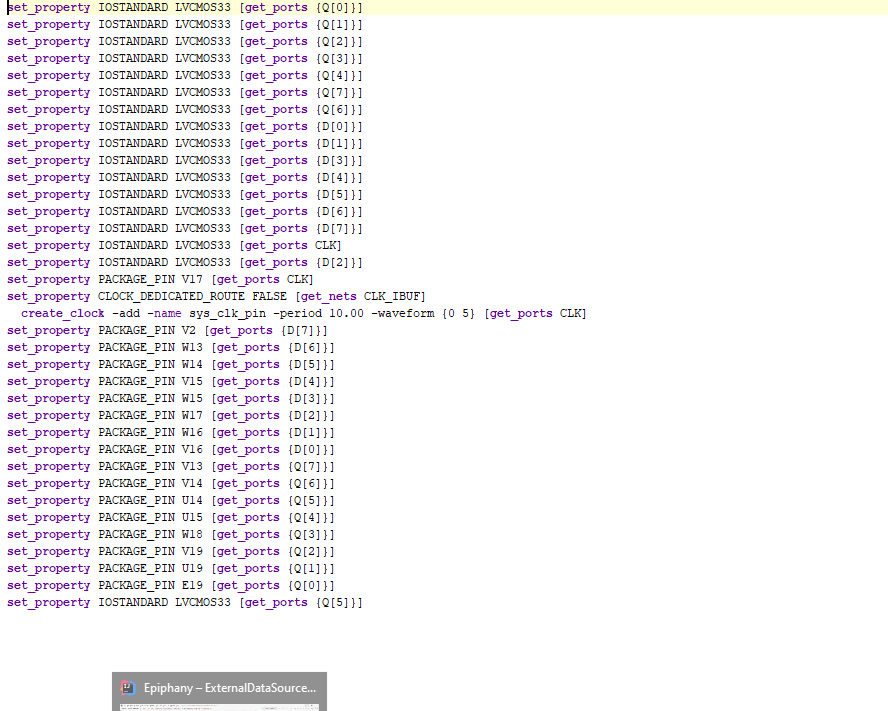
\includegraphics[width=1\textwidth]{8BitRegisterConstraints.png} % Include the image placeholder.png
\caption{8-Bit Register Constraints}
\end{center}
\end{figure}


\begin{figure}[h]
\begin{center}
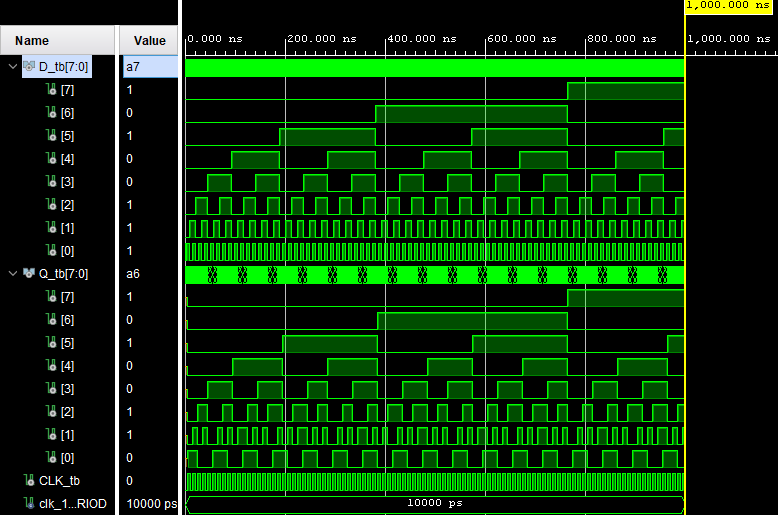
\includegraphics[width=1\textwidth]{8BitRegisterWaveForm.png} % Include the image placeholder.png
\caption{8-Bit Register Wavefrom}
\end{center}
\end{figure}


%----------------------------------------------------------------------------------------
%	SECTION 6
%----------------------------------------------------------------------------------------

\section{Feedback}
The biggest problem I had was introducing my board into this lab. I have the BASYS 3, so the pins were different.
Also, I wasnt able to readily identify which project part I needed, it was xc7a35tcpg236-1. Another obstucle I had to overcome 
was the abilty to set the clock to my SW0 pin/ override the default clock. 


%----------------------------------------------------------------------------------------
%	BIBLIOGRAPHY
%----------------------------------------------------------------------------------------

\bibliographystyle{apalike}

\bibliography{sample}

%----------------------------------------------------------------------------------------


\end{document}